%-----------------------------------------------------------------------
% flatPlate notes
%-----------------------------------------------------------------------
\documentclass[10pt]{article}
% \usepackage[bookmarks=true]{hyperref}  % this changes the page location !
\usepackage[bookmarks=true,colorlinks=true,linkcolor=blue]{hyperref}

% \input documentationPageSize.tex
\hbadness=10000 
\sloppy \hfuzz=30pt

% \voffset=-.25truein
% \hoffset=-1.25truein
% \setlength{\textwidth}{7in}      % page width
% \setlength{\textheight}{9.5in}    % page height

\usepackage{calc}
\usepackage[lmargin=.75in,rmargin=.75in,tmargin=.75in,bmargin=.75in]{geometry}

\input homeHenshaw

% \input{pstricks}\input{pst-node}
% \input{colours}
\newcommand{\blue}{\color{blue}}
\newcommand{\green}{\color{green}}
\newcommand{\red}{\color{red}}
\newcommand{\black}{\color{black}}


\usepackage{amsmath}
\usepackage{amssymb}

\usepackage{verbatim}
\usepackage{moreverb}

\usepackage{graphics}    
\usepackage{epsfig}    
\usepackage{calc}
\usepackage{ifthen}
\usepackage{float}
% the next one cause the table of contents to disappear!
% * \usepackage{fancybox}

\usepackage{makeidx} % index
\makeindex
\newcommand{\Index}[1]{#1\index{#1}}

\usepackage{tikz}
\usepackage{pgfplots}
\input trimFig.tex


% ---- we have lemmas and theorems in this paper ----
\newtheorem{assumption}{Assumption}
\newtheorem{definition}{Definition}

% \newcommand{\homeHenshaw}{/home/henshaw.0}

\newcommand{\Overture}{{\bf Over\-ture\ }}
\newcommand{\ogenDir}{\homeHenshaw/Overture/ogen}

\newcommand{\cgDoc}{\homeHenshaw/cgDoc}
\newcommand{\vpDir}{\homeHenshaw/cgDoc/ins/viscoPlastic}

\newcommand{\ovFigures}{\homeHenshaw/OvertureFigures}
\newcommand{\obFigures}{\homeHenshaw/res/OverBlown/docFigures}  % for figures
\newcommand{\convDir}{\homeHenshaw/cgDoc/ins/tables}
\newcommand{\insDocDir}{\homeHenshaw/cgDoc/ins}

% *** See http://www.eng.cam.ac.uk/help/tpl/textprocessing/squeeze.html
% By default, LaTeX doesn't like to fill more than 0.7 of a text page with tables and graphics, nor does it like too many figures per page. This behaviour can be changed by placing lines like the following before \begin{document}

\renewcommand\floatpagefraction{.9}
\renewcommand\topfraction{.9}
\renewcommand\bottomfraction{.9}
\renewcommand\textfraction{.1}   
\setcounter{totalnumber}{50}
\setcounter{topnumber}{50}
\setcounter{bottomnumber}{50}

\begin{document}

\input wdhDefinitions.tex

\def\comma  {~~~,~~}
\newcommand{\uvd}{\mathbf{U}}
\def\ud     {{    U}}
\def\pd     {{    P}}
\def\calo{{\cal O}}

\newcommand{\mbar}{\bar{m}}
\newcommand{\Rbar}{\bar{R}}
\newcommand{\Ru}{R_u}         % universal gas constant
% \newcommand{\Iv}{{\bf I}}
% \newcommand{\qv}{{\bf q}}
\newcommand{\Div}{\grad\cdot}
\newcommand{\tauv}{\boldsymbol{\tau}}
\newcommand{\thetav}{\boldsymbol{\theta}}
% \newcommand{\omegav}{\mathbf{\omega}}
% \newcommand{\Omegav}{\mathbf{\Omega}}

\newcommand{\Omegav}{\boldsymbol{\Omega}}
\newcommand{\omegav}{\boldsymbol{\omega}}
\newcommand{\sigmav}{\boldsymbol{\sigma}}
\newcommand{\cm}{{\rm cm}}

\newcommand{\ds}{\Delta s}
\newcommand{\dsbl}{\ds_{\rm bl}}


\newcommand{\sumi}{\sum_{i=1}^n}
% \newcommand{\half}{{1\over2}}
\newcommand{\dt}{{\Delta t}}

\def\ff {\tt} % font for fortran variables

% define the clipFig commands:
%% \input clipFig.tex

\newcommand{\Bc}{{\mathcal B}}
\newcommand{\Dc}{{\mathcal D}}
\newcommand{\Ec}{{\mathcal E}}
\newcommand{\Fc}{{\mathcal F}}
\newcommand{\Gc}{{\mathcal G}}
\newcommand{\Hc}{{\mathcal H}}
\newcommand{\Ic}{{\mathcal I}}
\newcommand{\Jc}{{\mathcal J}}
\newcommand{\Lc}{{\mathcal L}}
\newcommand{\Nc}{{\mathcal N}}
\newcommand{\Pc}{{\mathcal P}}
\newcommand{\Rc}{{\mathcal R}}
\newcommand{\Sc}{{\mathcal S}}

\newcommand{\bogus}[1]{}  % removes is argument completely

\vspace{5\baselineskip}
\begin{flushleft}
{\Large
Some results for a flat plate boundary layer
}

\end{flushleft}


% -------------------------------------------------------------------------------
\subsection{Flat plate boundary layer} \label{sec:flatPlateBoundaryLayer}


In this section we consider the computation of the flow over a flat plate.
The plate is horizontal and starts at $(x,y)=(0,0)$.
The boundary layer solution is an approximation solution to the laminar flow past a flat plate. The
solution  is given by (derived by Prandtl's student Blasius)
\begin{align*}
   & u = U f'(\eta), \\
   & v = \half \sqrt{\frac{\nu U}{x}} \Big( \eta f' - f \Big), 
\end{align*}
where the similiarity variable $\eta$ is defined as
\begin{align*}
   & \eta = y\, \sqrt{\frac{U}{\nu x}},
\end{align*}
and where $f$ satisfies the 3rd order ODE:
\begin{align*}
   & f f'' + 2 f ''' = 0, \qquad f(0)=0, ~ f'(0)=0, ~ f'(\infty)=1.
\end{align*}
This problem can be solved as a shooting problem with initial condition
\begin{align*}
   f''(0) \approx 0.3320573362151946
\end{align*}
Note that $v$ only makes sense if $\sqrt{\frac{\nu U}{x}}$ is small which implies $\nu$ is small
and $x$ is not too small (i.e. we cannot evaluate the solution too close to the leading edge). 
We thus start the computation at some offset value $x=x_0$

The thickness of the boundary layer is
\begin{align*}
   \delta(x) \approx C_\delta \sqrt{\frac{\nu x}{U}} , 
\end{align*}
where $C_\delta\approx 5$ for $u\approx .99 U$ on the edge of the boundary layer. 
The thickness of the boundary layer at inflow will this be $\delta(x_0)$ and we should therefore have
enough grid points to resolve this layer. 

This boundary solution is evaluated in the class {\tt BoundaryLayerProfile}.
Since the solution is only approximate the errors will not go zero as the mesh is refined.
The errors should become smaller, however, as $\sqrt{\frac{\nu U}{x_0}} \rightarrow 0$, e.g. 
if $\nu\rightarrow 0$ or $x_0\rightarrow\infty$. 


The cgins script {\tt flatPlate.cmd} can be used to solve for the flow past a flat plate.

Figure~\ref{fig:boundaryLayer} shows results for the flat plate boundary layer for the
case $\nu=10^{-3}$, $x_0=5$. 


{
\newcommand{\figWidthp}{8.cm}
\newcommand{\trimfig}[2]{\trimPlotb{#1}{#2}{.0}{.0}{.0}{.0}}
\begin{figure}[hbt]
\begin{center}
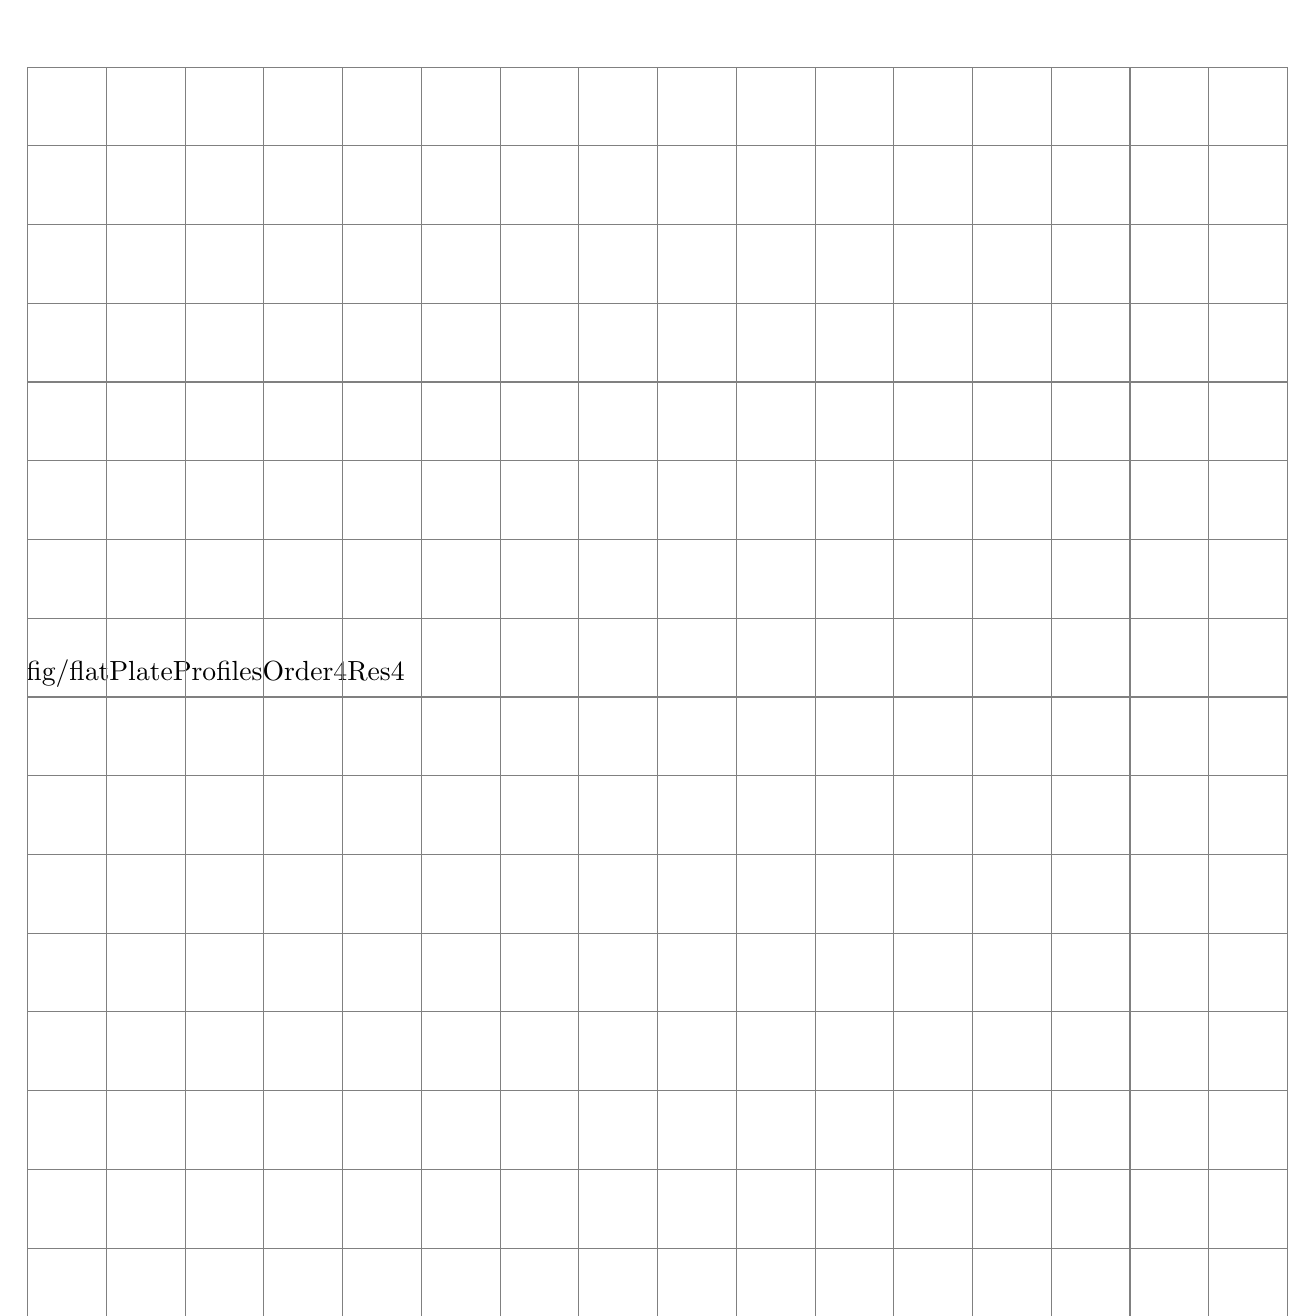
\begin{tikzpicture}[scale=1]
  \useasboundingbox (0,.5) rectangle (16.,16.5);  % set the bounding box (so we have less surrounding white space)
%
  \draw ( 0.0, 8) node[anchor=south west,xshift=-4pt,yshift=+0pt] {\trimfig{fig/flatPlateProfilesOrder4Res4}{\figWidthp}};
%  \draw ( 8.0, 8) node[anchor=south west,xshift=-4pt,yshift=+0pt] {\trimfig{fig/pump8i0p5pt0p5}{\figWidthp}};
%  \draw ( 0.0, 0) node[anchor=south west,xshift=-4pt,yshift=+0pt] {\trimfig{fig/pump8i0p5SLt4p0}{\figWidthp}};
%  \draw ( 8.0, 0) node[anchor=south west,xshift=-4pt,yshift=+0pt] {\trimfig{fig/pump8i0p5pt4p0}{\figWidthp}};
 % \draw (current bounding box.south west) rectangle (current bounding box.north east);
% grid:
 \draw[step=1cm,gray] (0,0) grid (16,16);
\end{tikzpicture}
\end{center}
  \caption{Flat plate boundary layer. Top left: Results from IM24, $\nu=10^{-3}$, grid $\Gc_{fp}^{(4)}$, profiles at $x=3$. }
  \label{fig:boundaryLayer}
\end{figure}
}





\end{document}
